% vim: filetype=tex spell

\chapter{Offset Plots}

\label{ch:offplot}

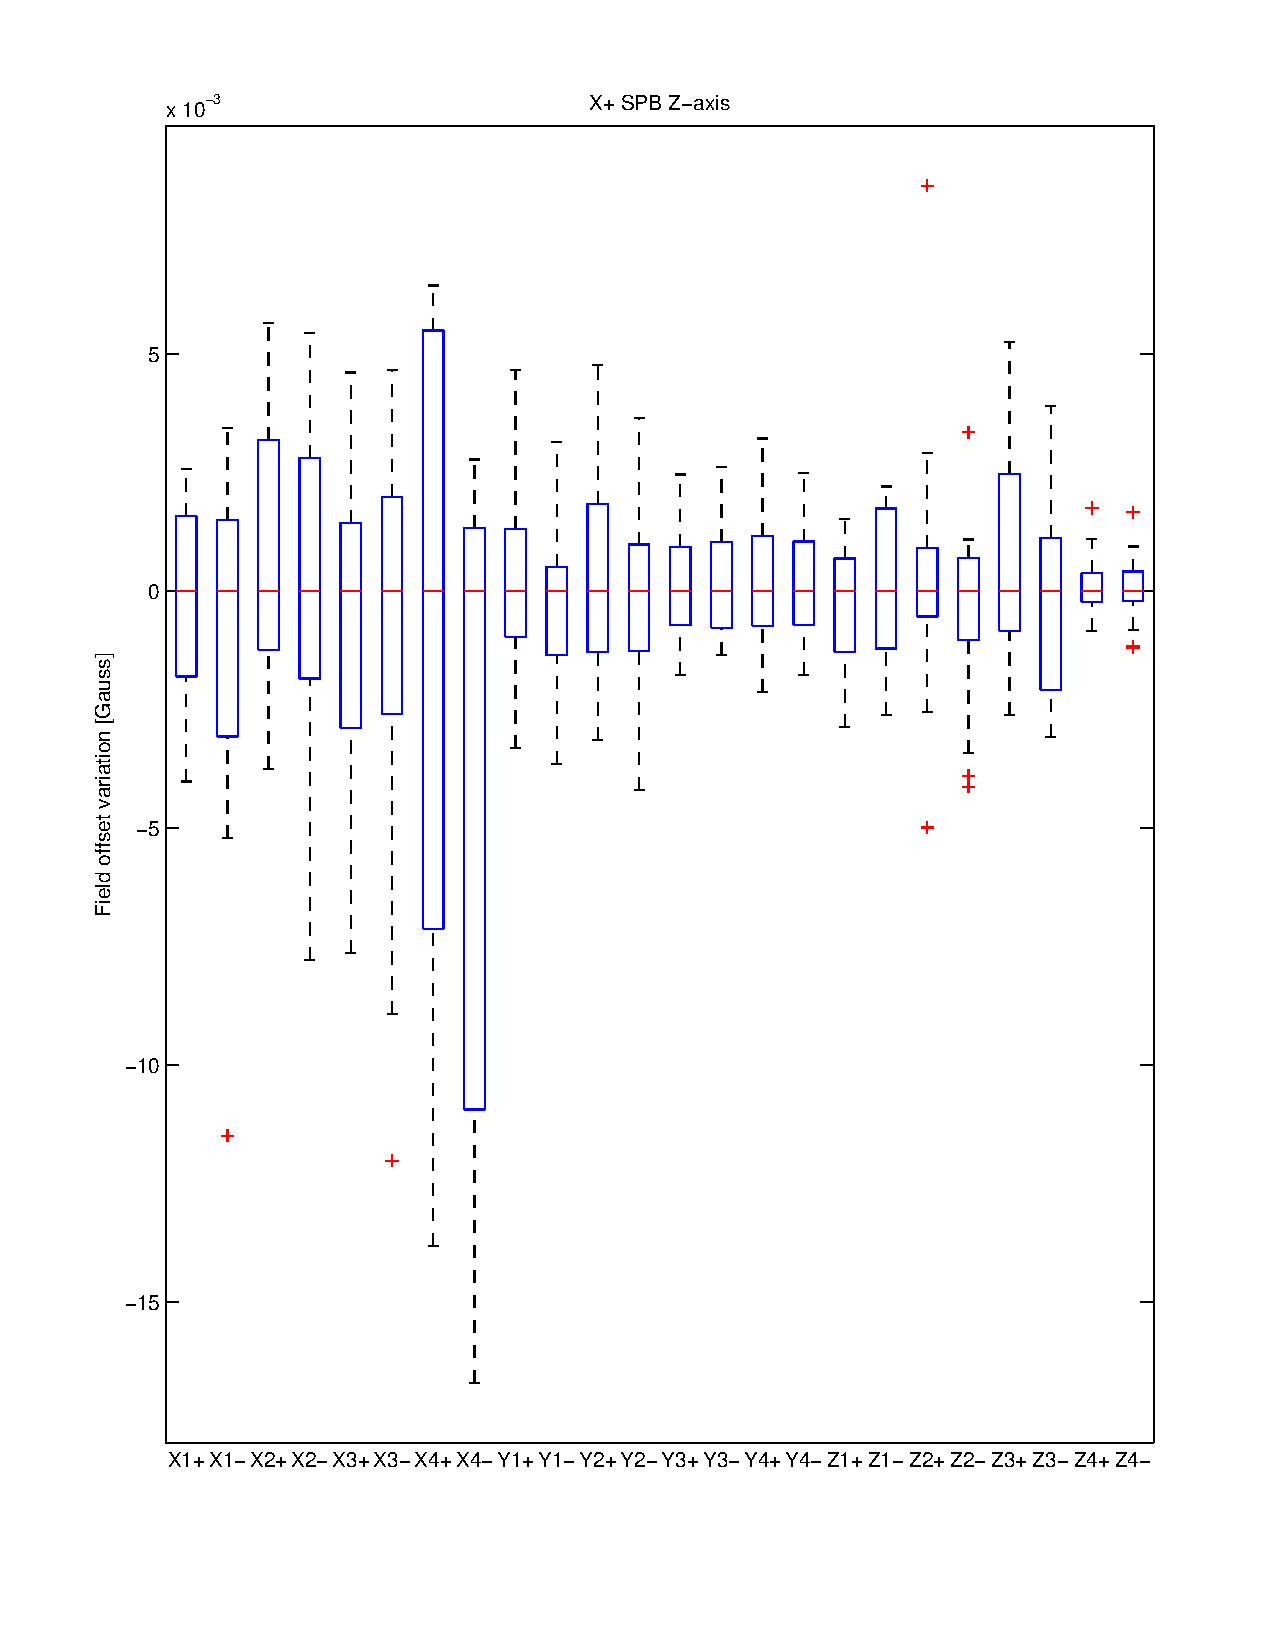
\includegraphics[width=\linewidth]{torqueOffsets_X+SPB-Z}

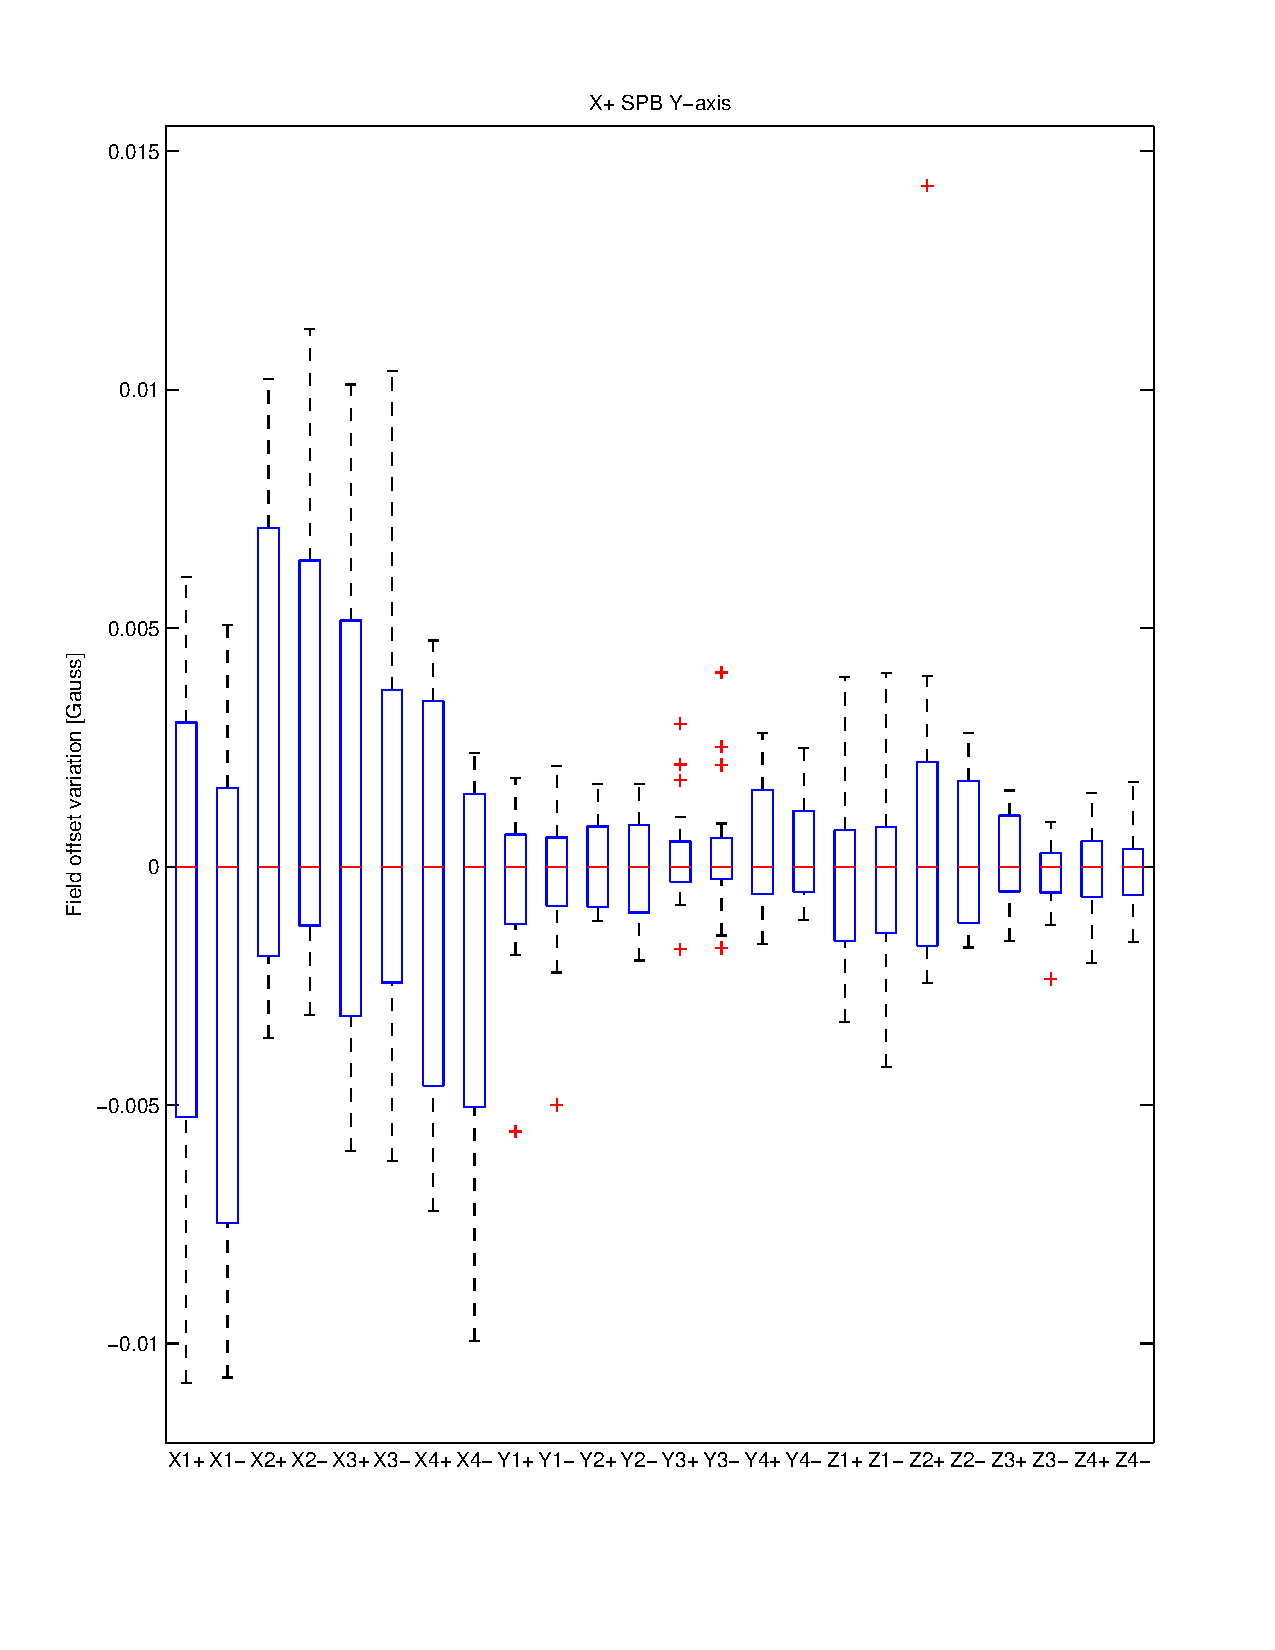
\includegraphics[width=\linewidth]{torqueOffsets_X+SPB-Y}


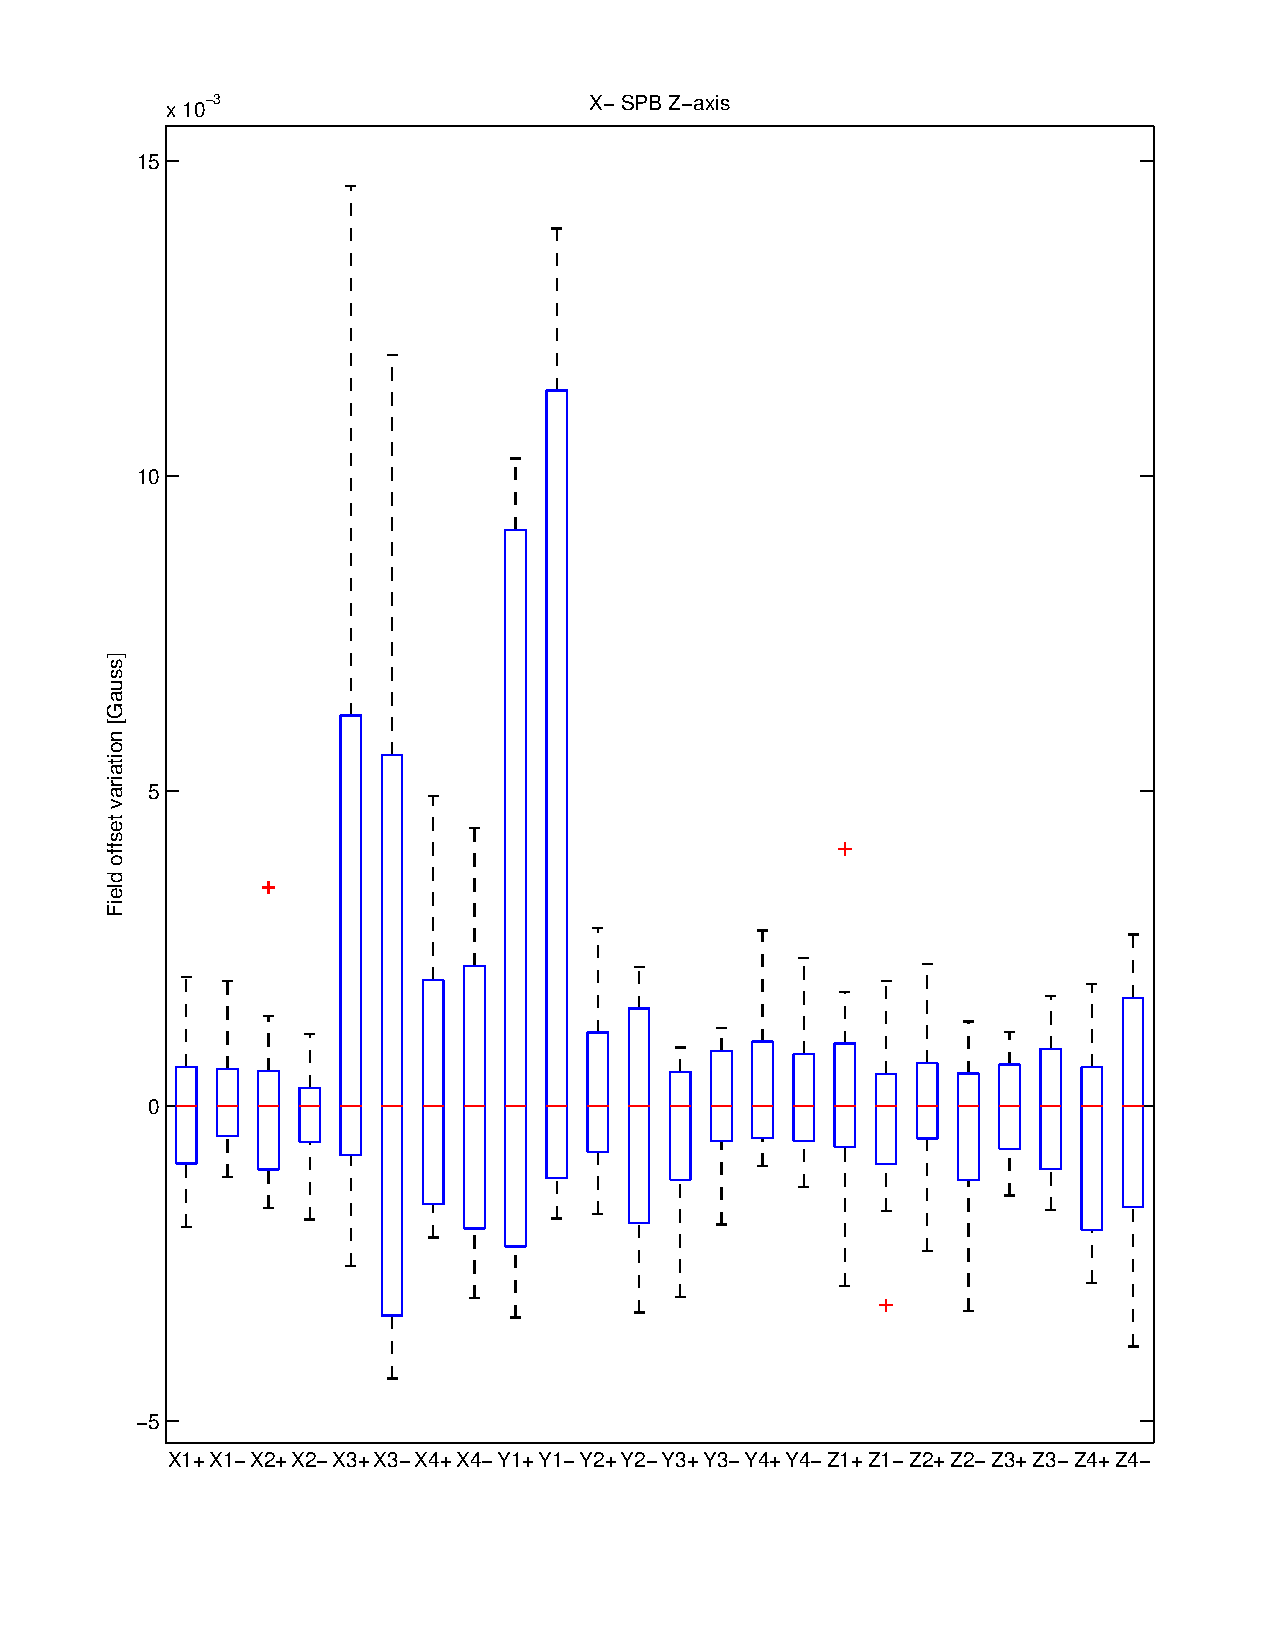
\includegraphics[width=\linewidth]{torqueOffsets_X-SPB-Z}

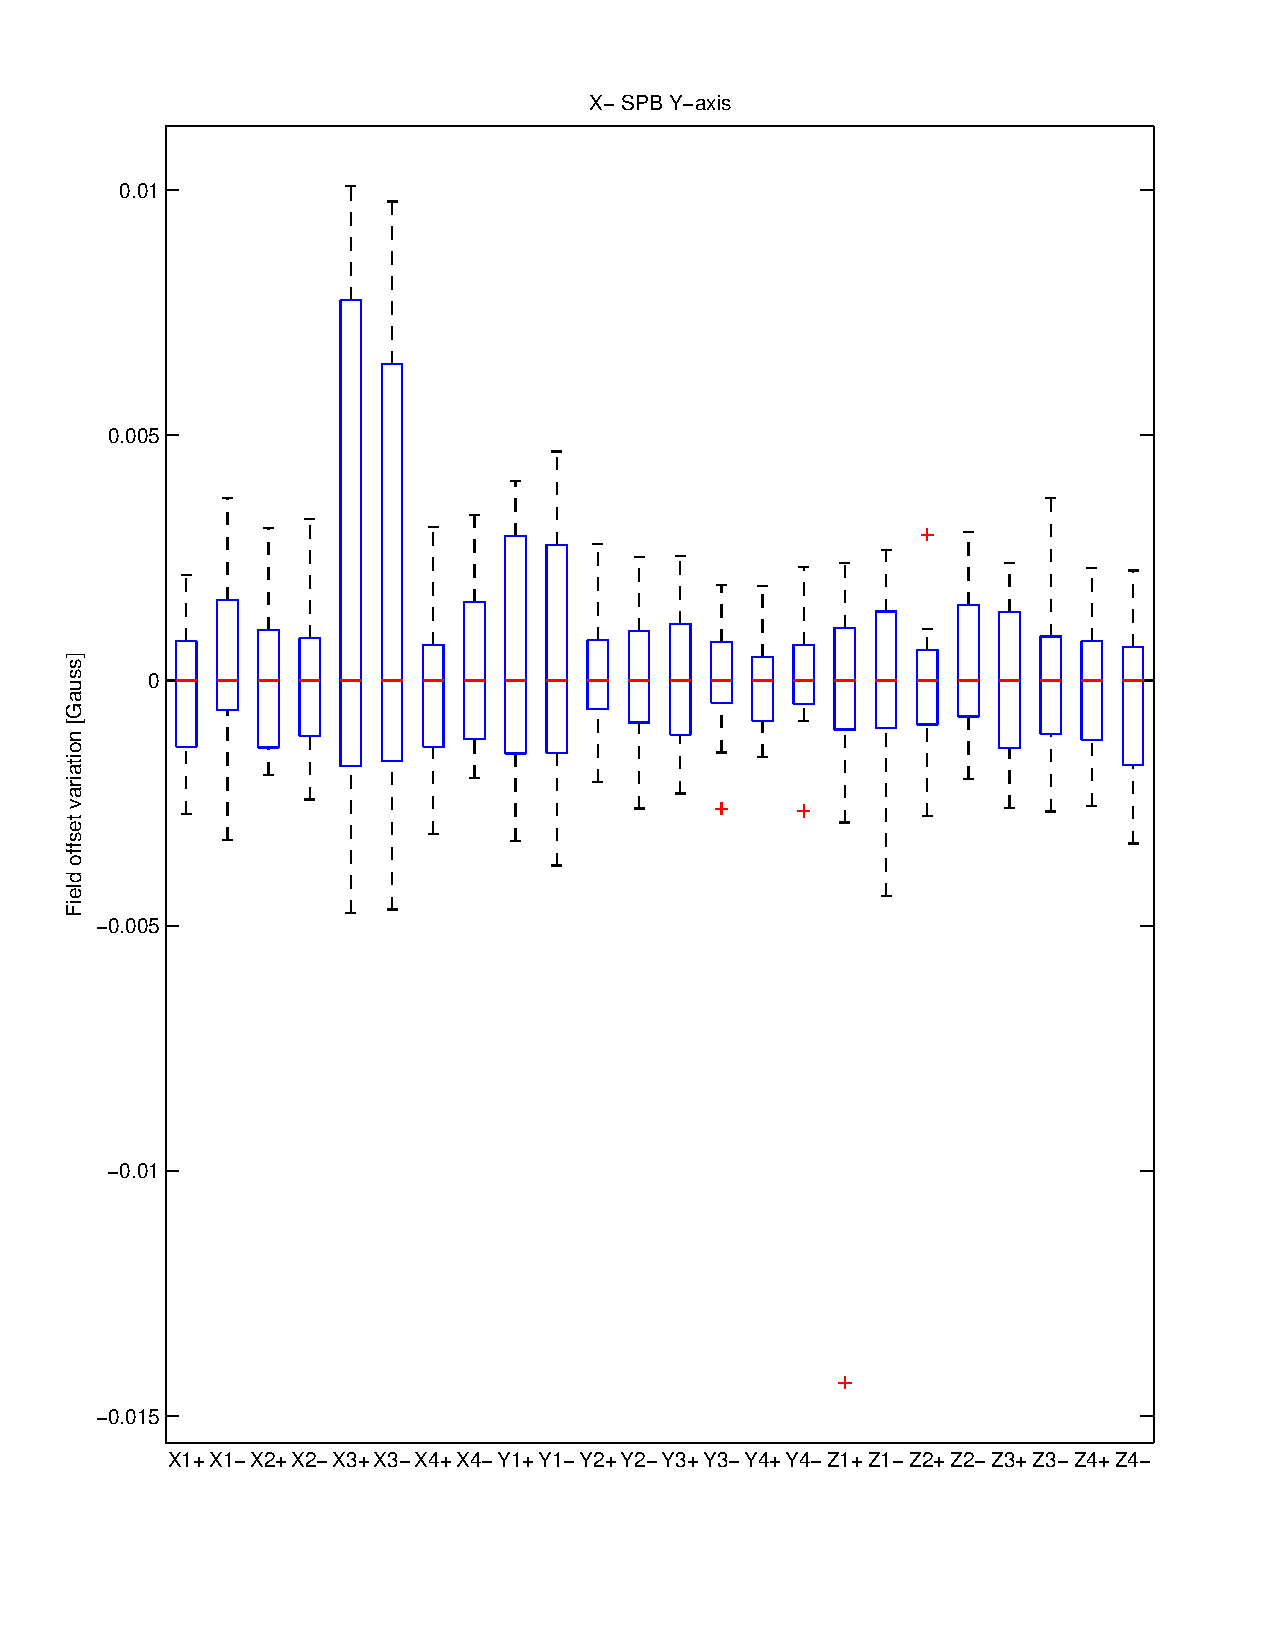
\includegraphics[width=\linewidth]{torqueOffsets_X-SPB-Y}


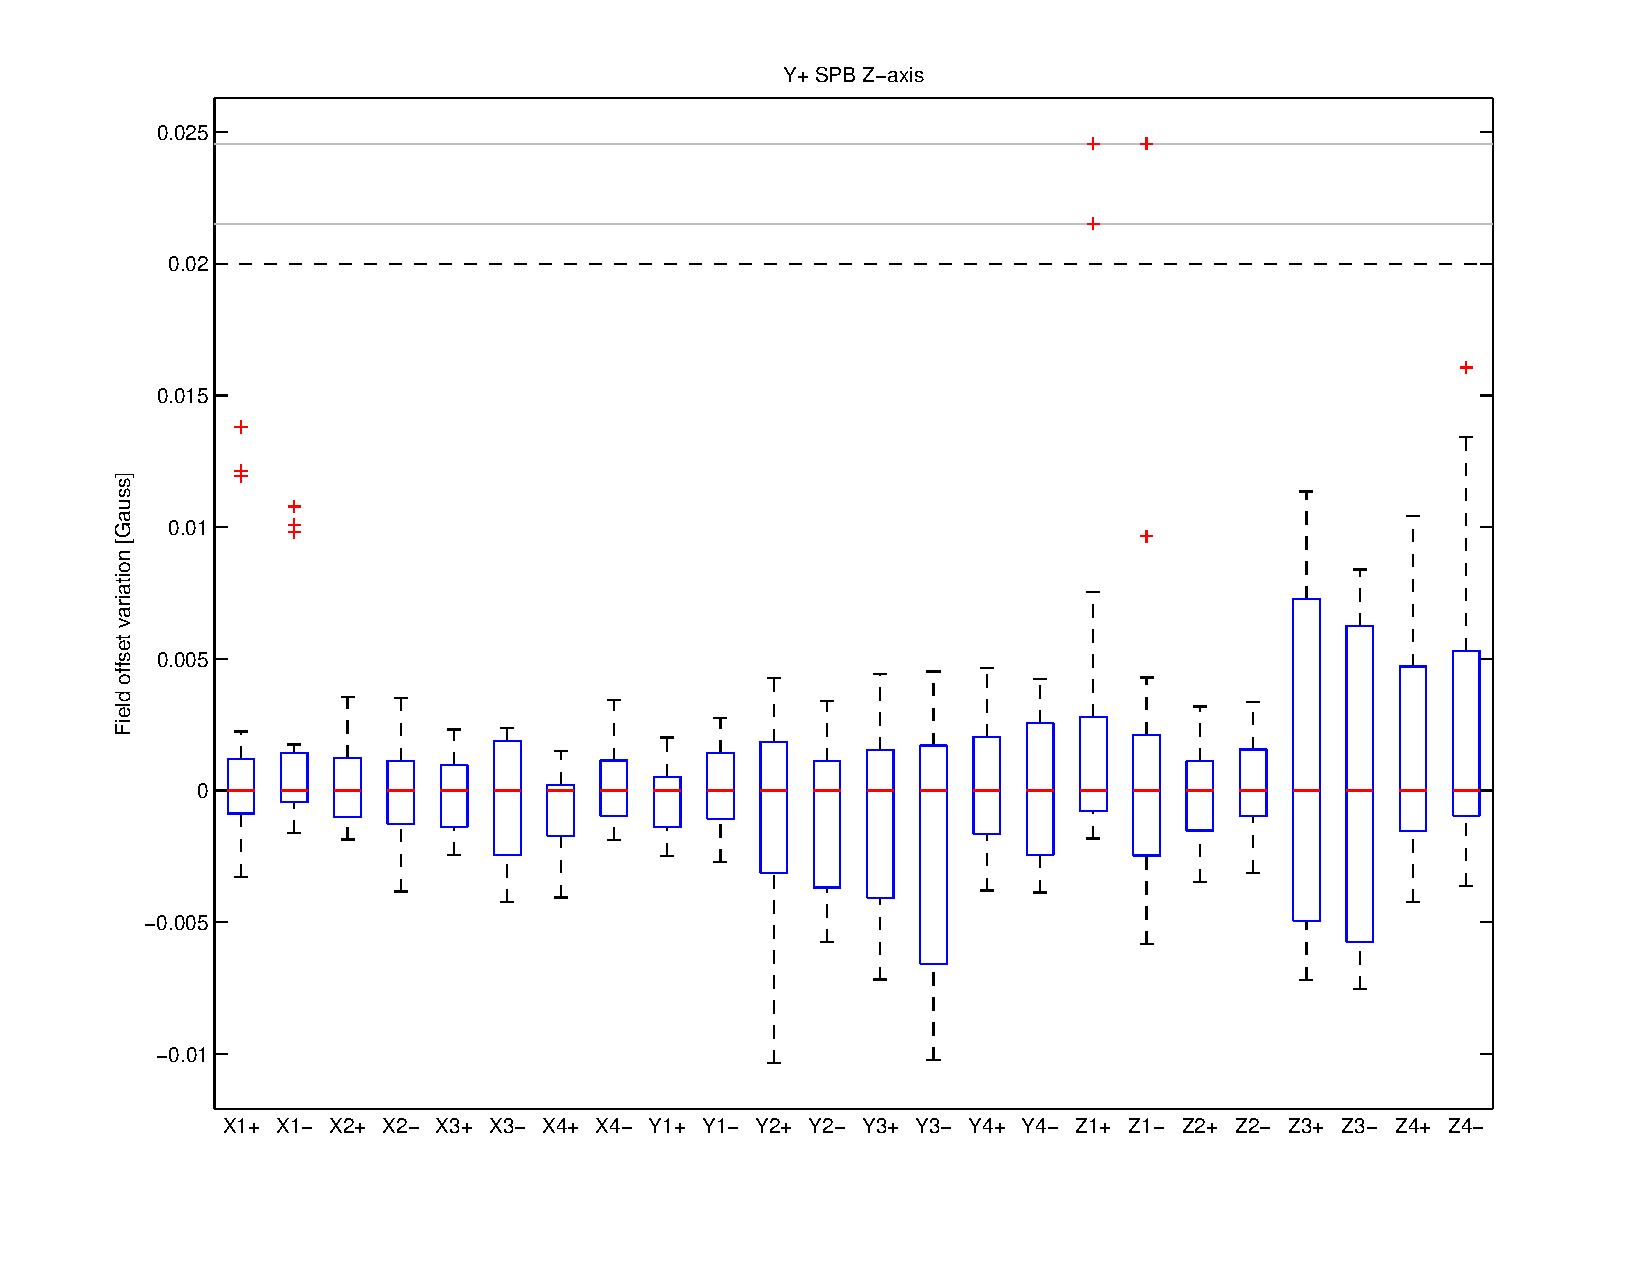
\includegraphics[width=\linewidth]{torqueOffsets_Y+SPB-Z}

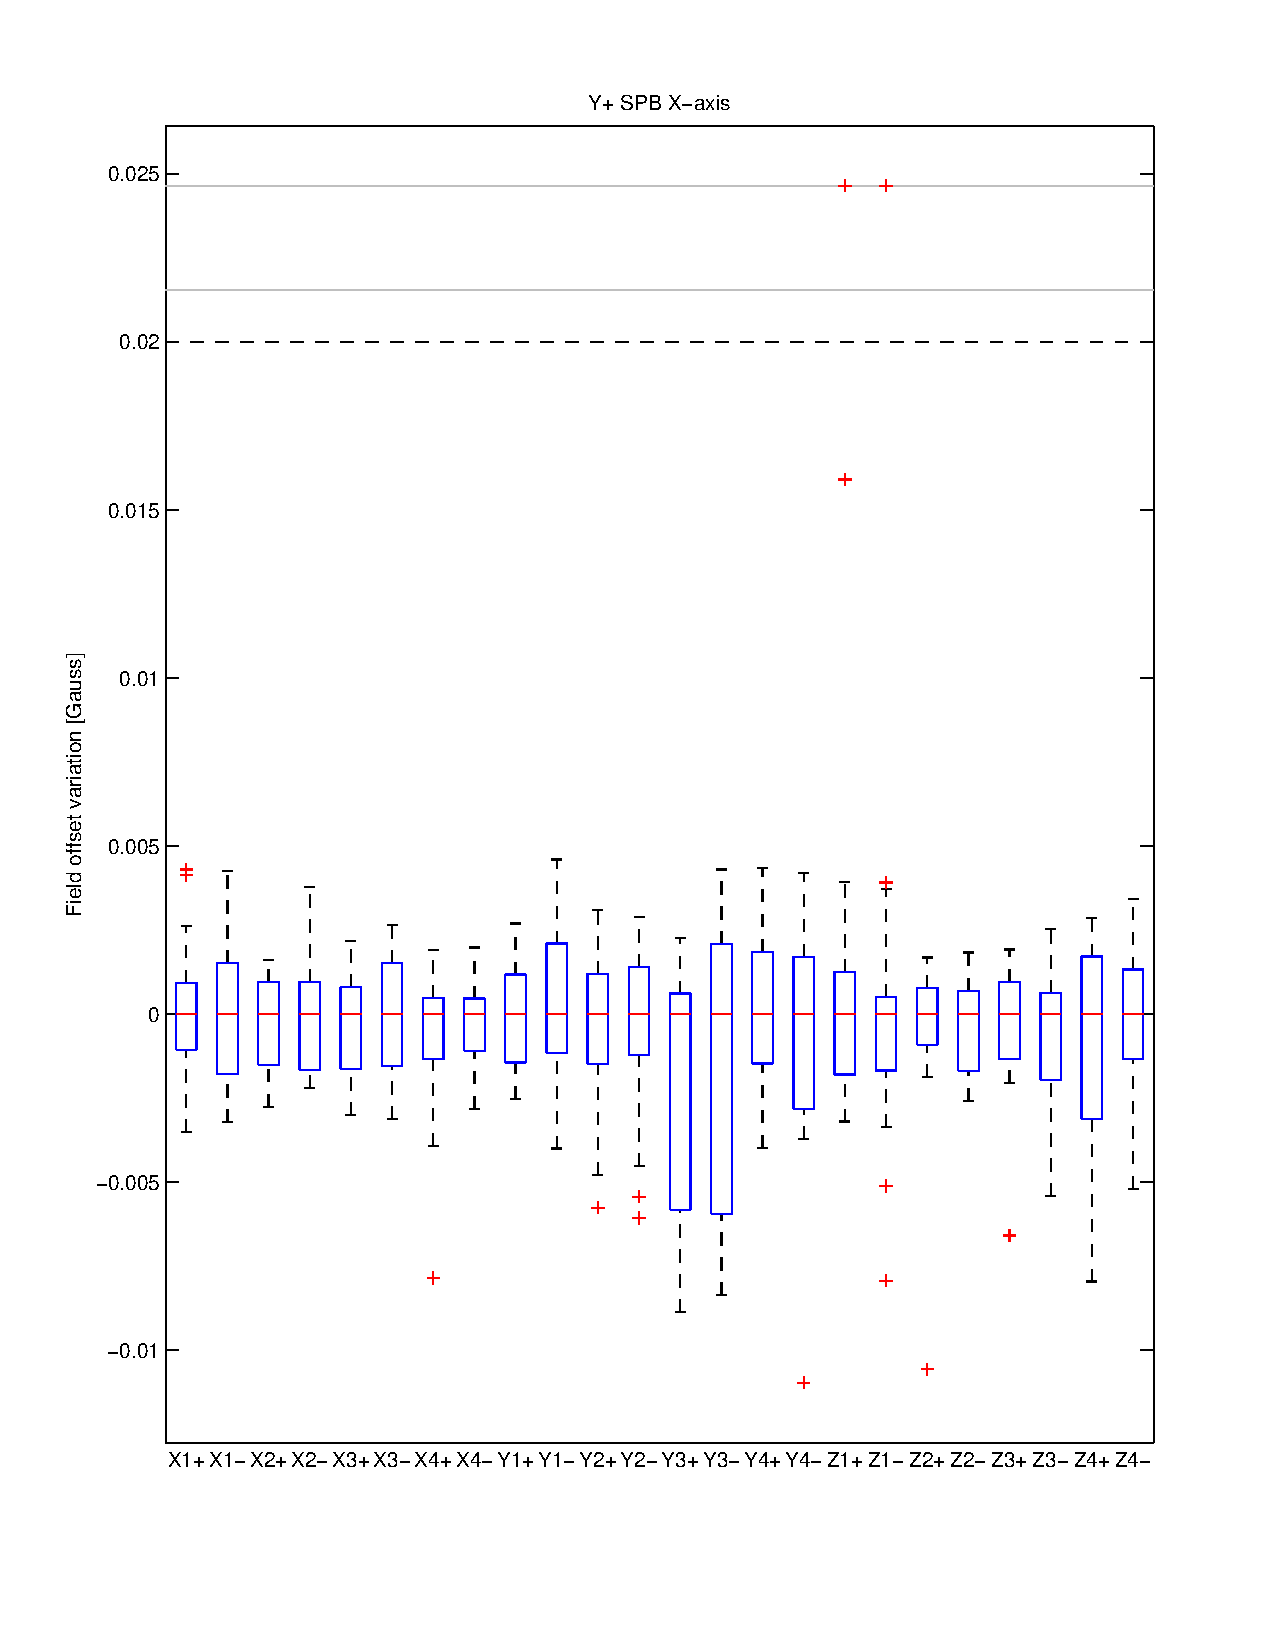
\includegraphics[width=\linewidth]{torqueOffsets_Y+SPB-X}


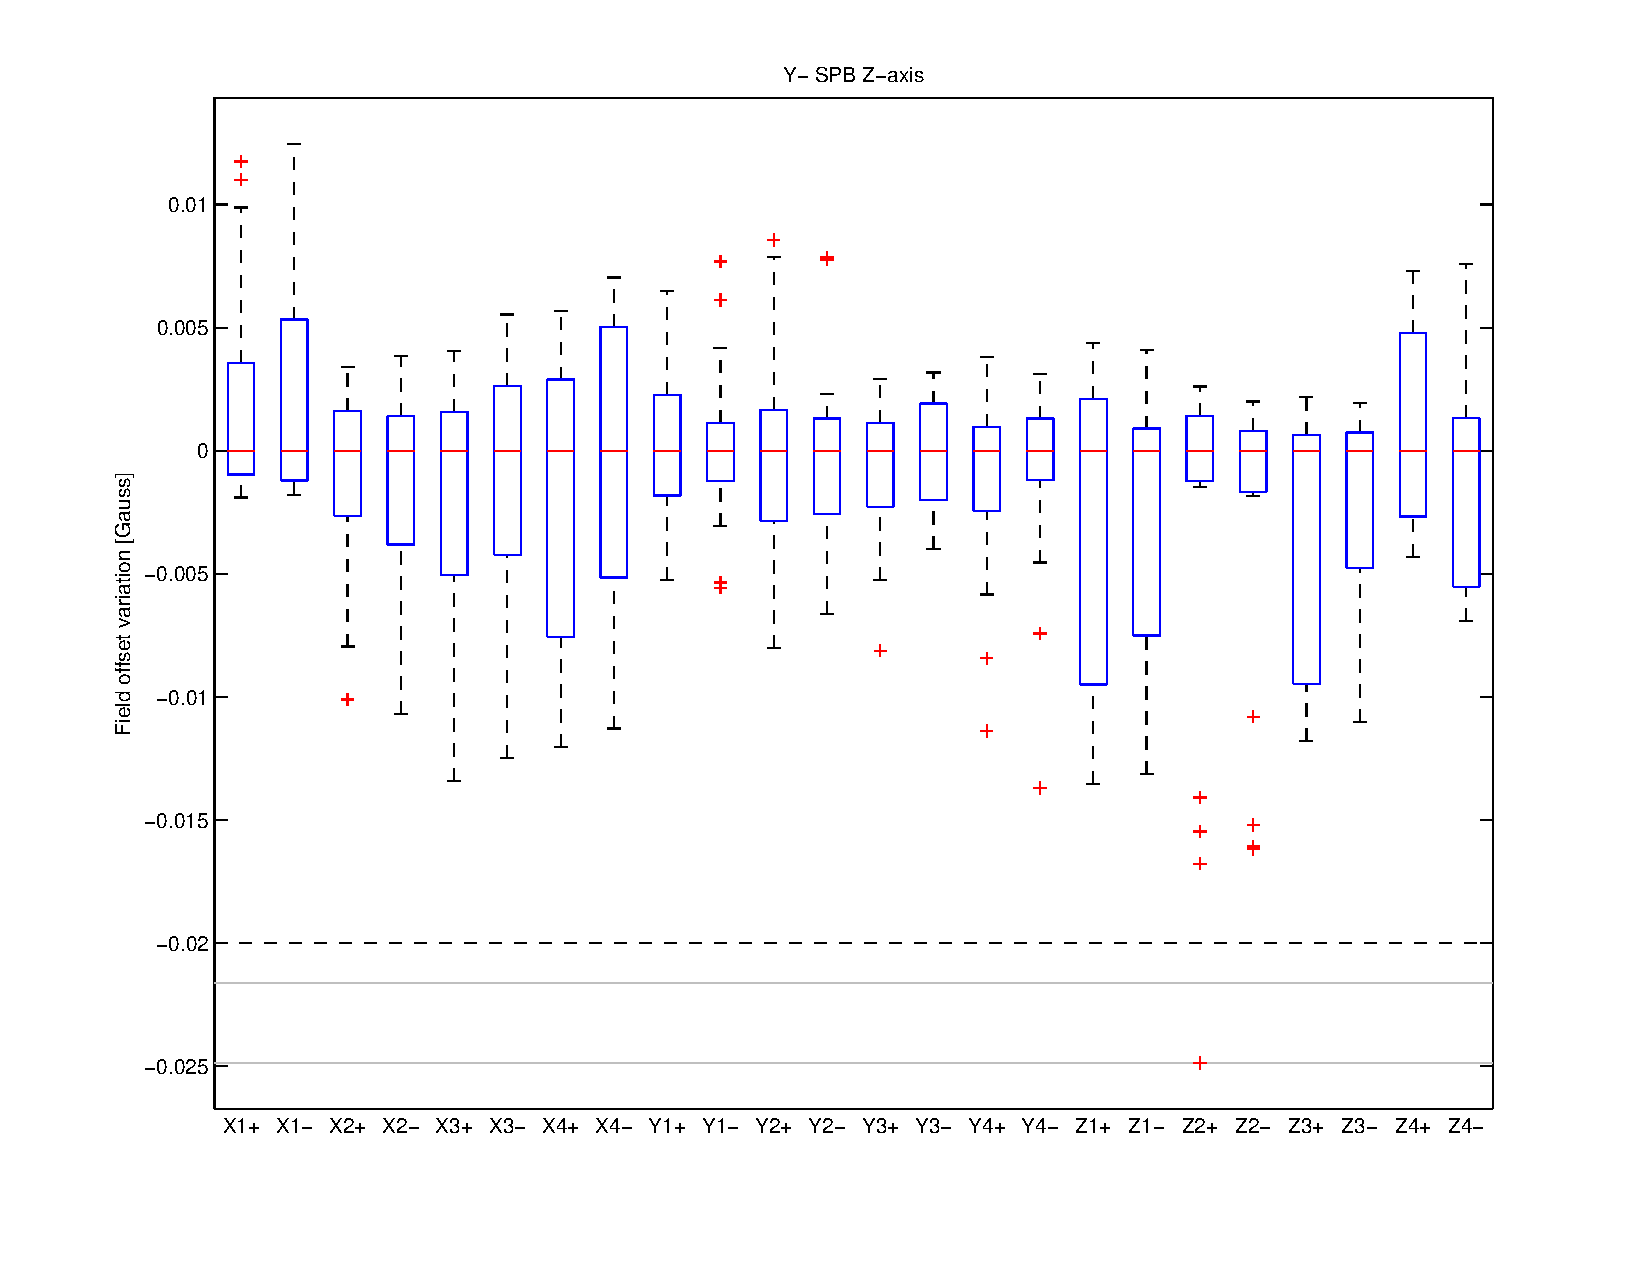
\includegraphics[width=\linewidth]{torqueOffsets_Y-SPB-Z}

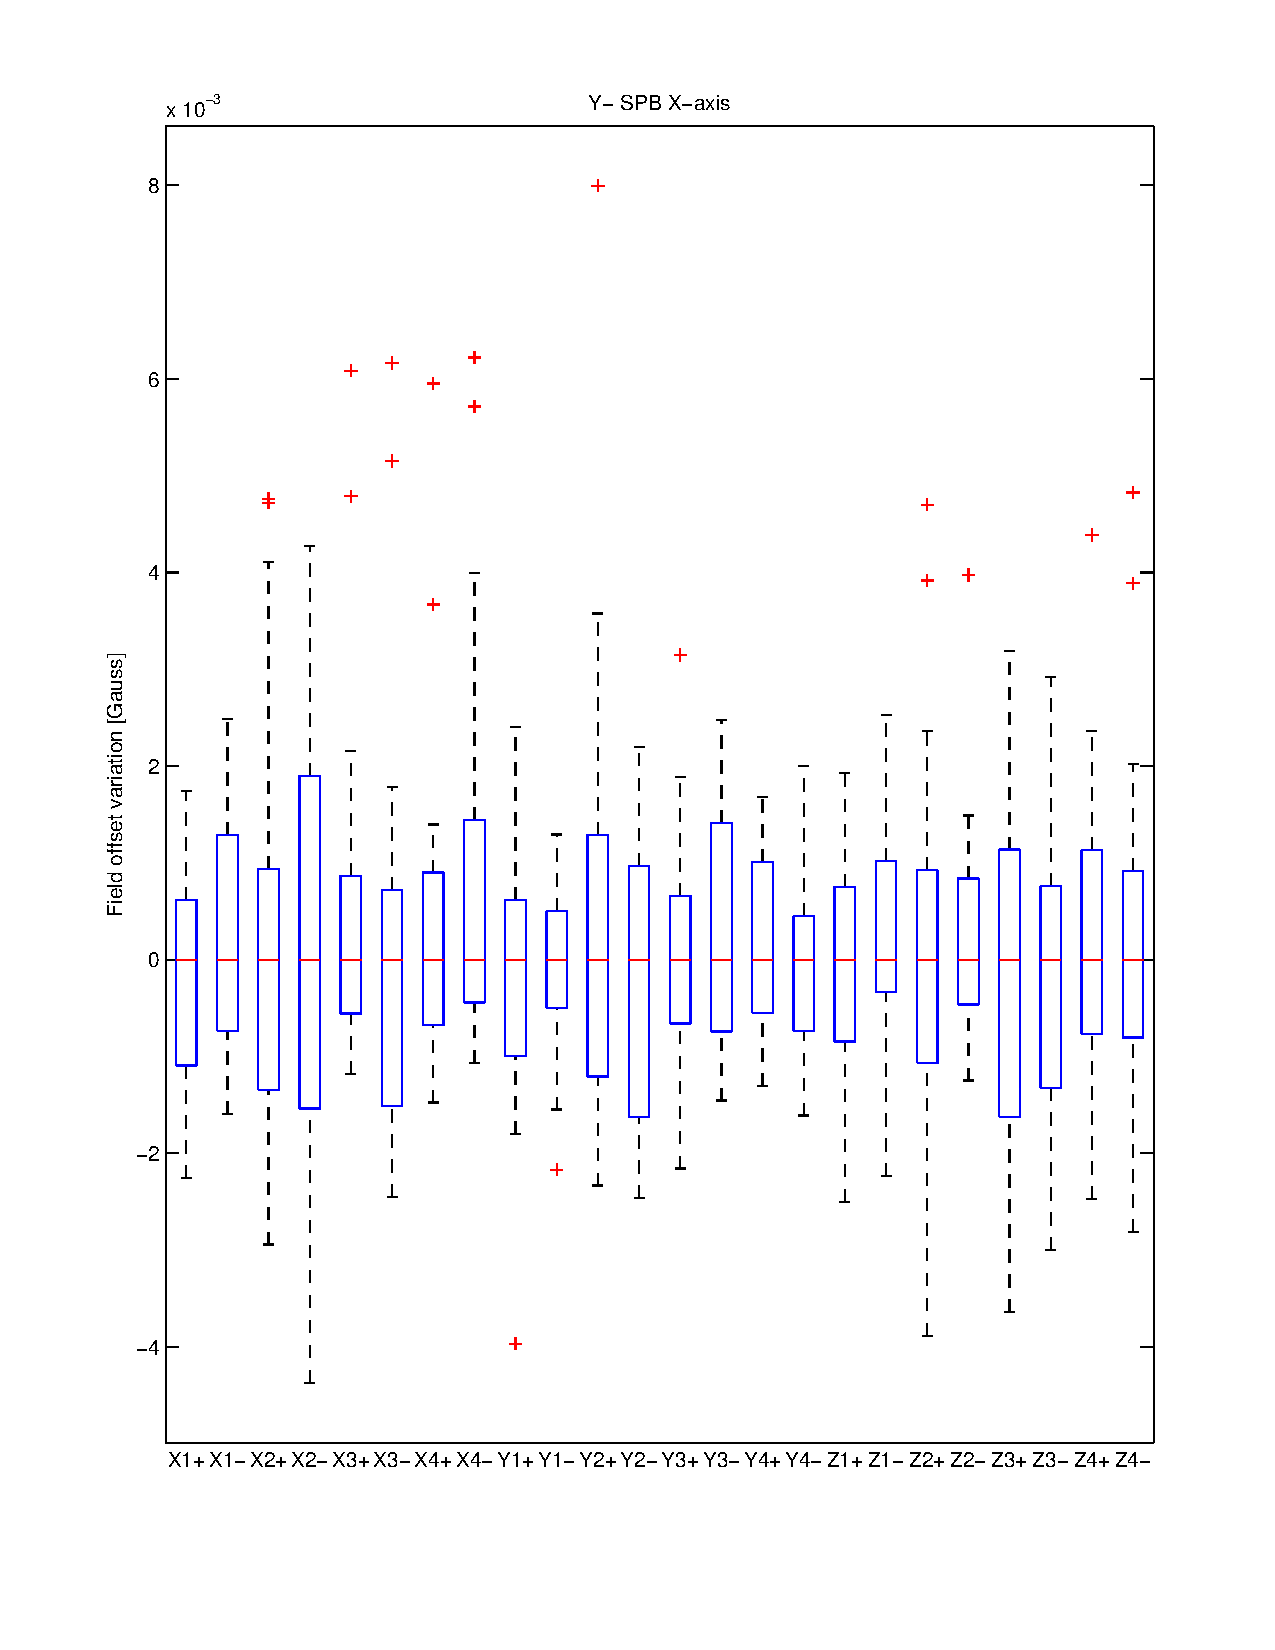
\includegraphics[width=\linewidth]{torqueOffsets_Y-SPB-X}


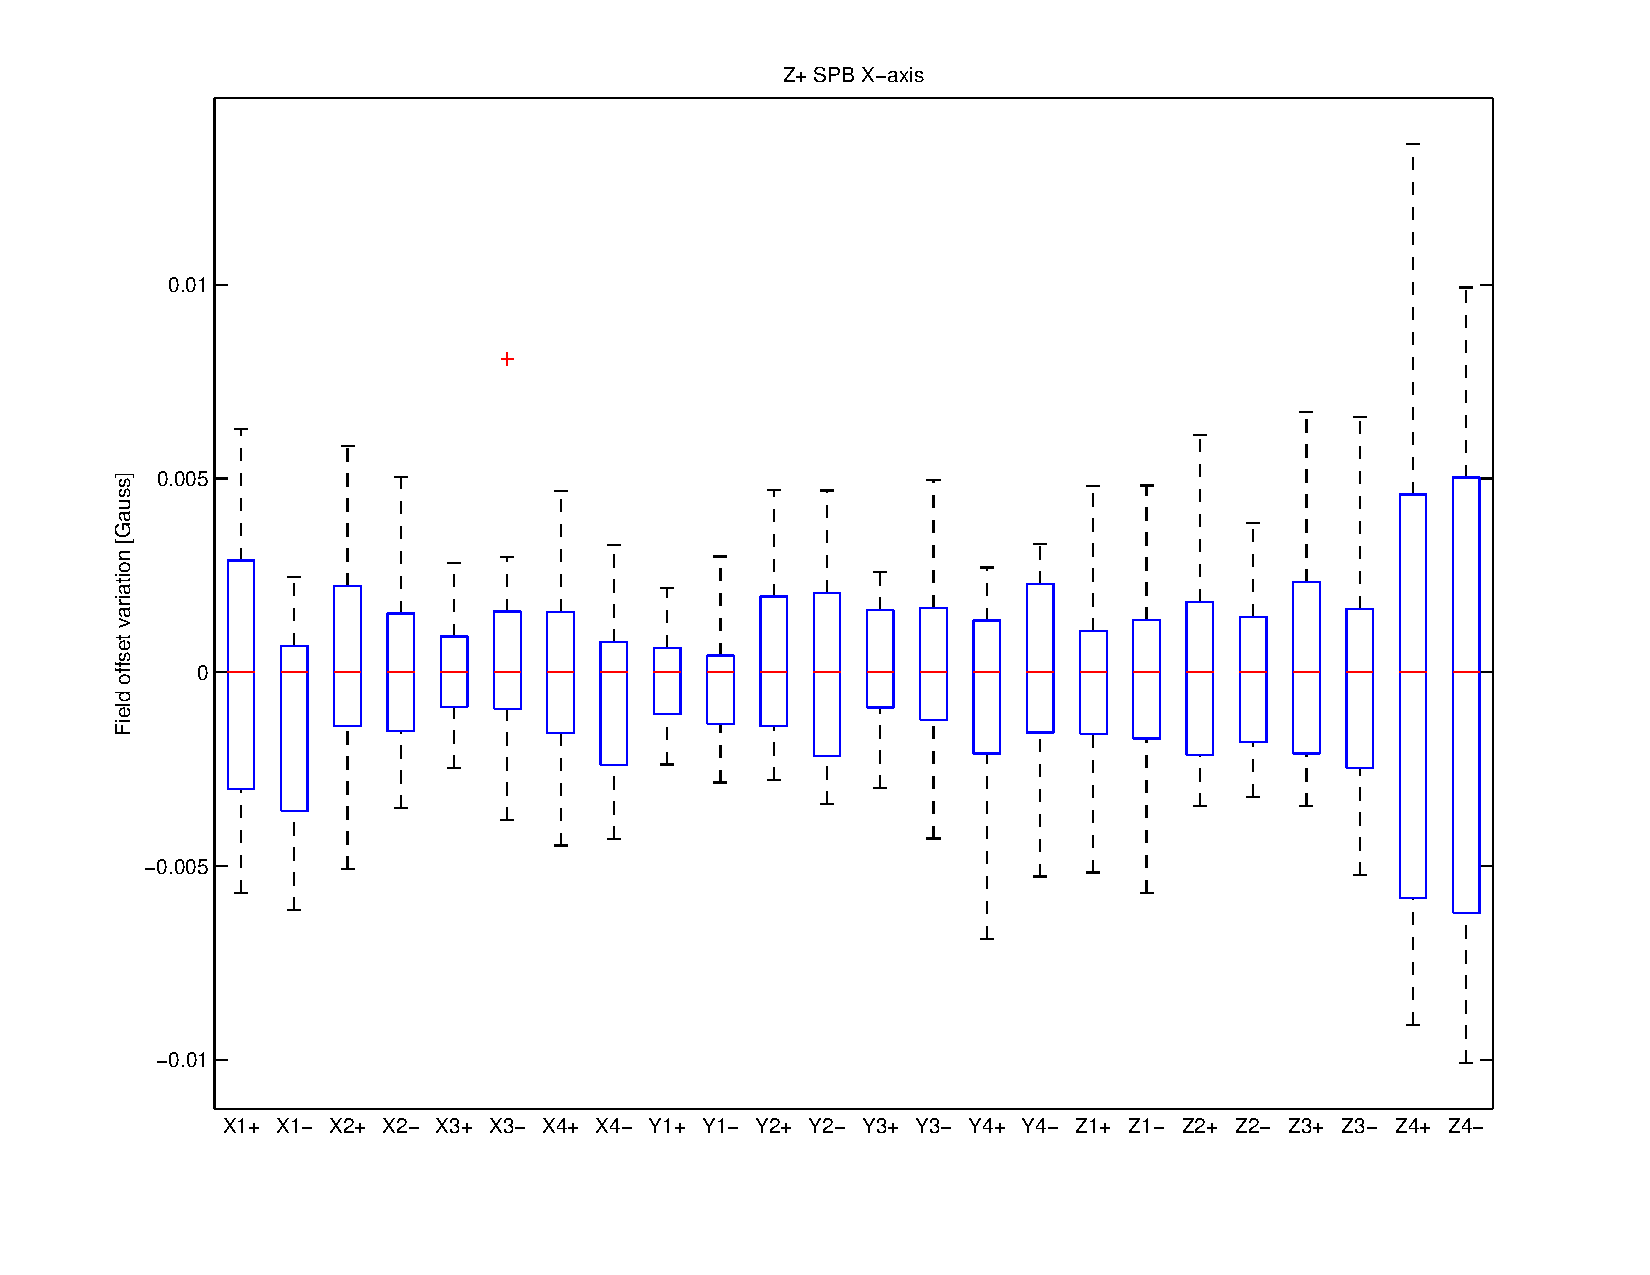
\includegraphics[width=\linewidth]{torqueOffsets_Z+SPB-X}

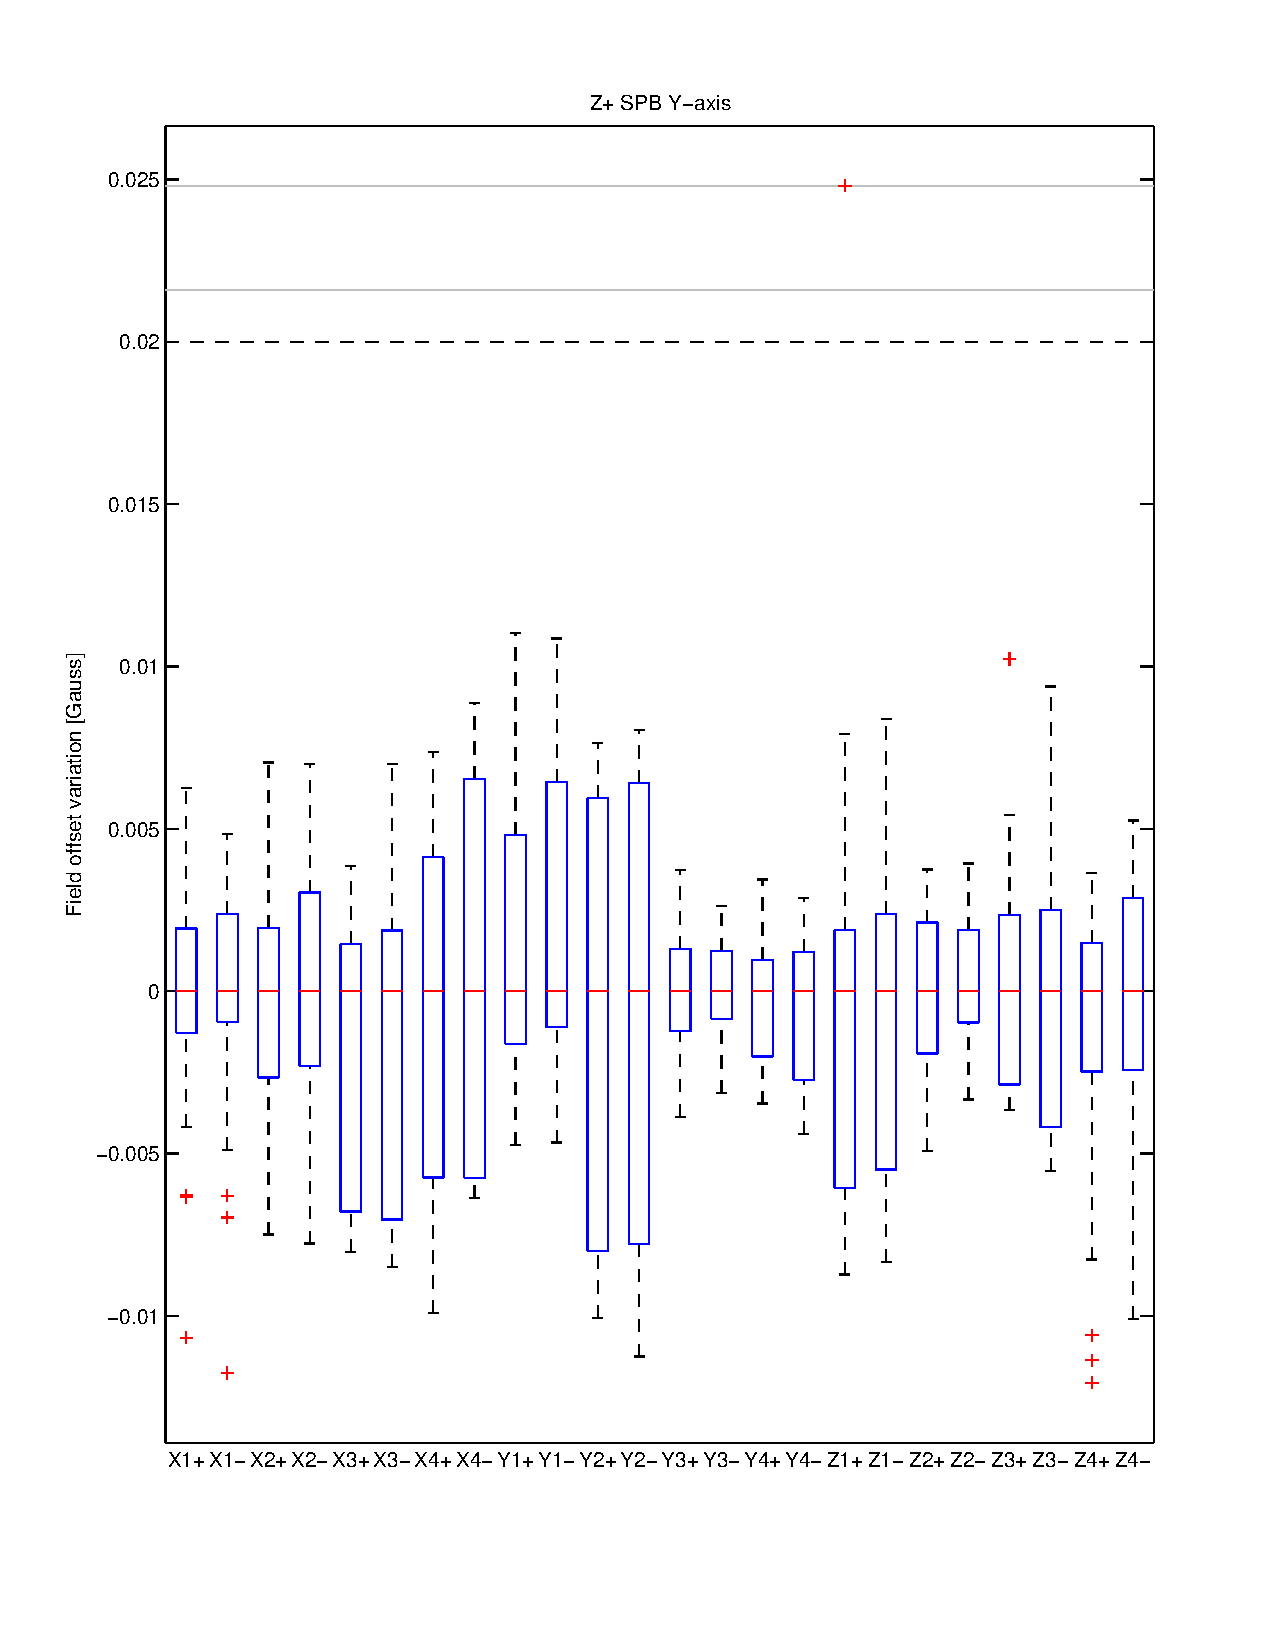
\includegraphics[width=\linewidth]{torqueOffsets_Z+SPB-Y}

